\section{Proposed Design}
\label{section:propeseddesign}
I propose instrumenting a wireless network to enforce authorization through integration with an
OAuth provider (Facebook). I will prototype a simple authorization scheme to allow the network
owner's friends access to the network. To create the authentication and authorization flow, I will
program a dual-band OpenWRT router to have an open SSID with a captive portal where the user will
use OAuth with Facebook to prove to the router who they are. At setup time, the network owner will
integrate the router with their list of Facebook friends. As users present themselves to the router,
if they are found to be in the owner's list of friends, they will be presented temporary credentials
to the second, WPA-encrypted SSID. Rather than take on the challenge of creating per-user keys on
the encrypted SSID, I will simply automate the resetting of the key to some frequent interval, such
as 1-2 times a day.

While my initial prototype will be fairly manual, it is meant to be a proof of concept. Should this
idea prove itself, my proposal is to publish the implementation as open-source router firmware and
open-source client apps/services to automate the handshaking. By open-sourcing the implementation,
router manufacturers could include the software in their products and device OS's could be modified
to implement the client-side automation.

\subsection{Handshaking}
Here, I show \ref{fig:handshake} and then describe the steps and actions taken by the network owner, user(s), and instrumented router to
achieve OAuth-secured wireless network.

\begin{figure}[ht!]
\centering
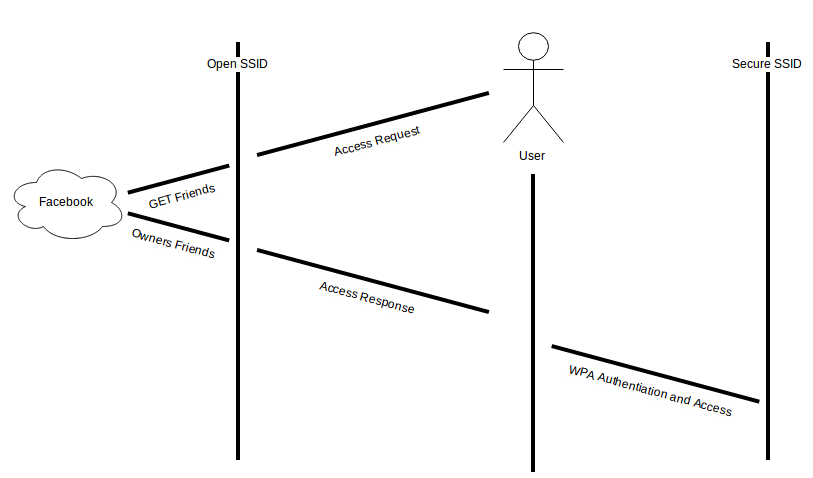
\includegraphics[width=90mm]{fig/handshake.png}
\caption{Handshake process shown visually}
\label{fig:handshake}
\end{figure}

\begin{description}
\item{Setup:} First, the network owner will authenticate the router on her behalf with Facebook,
granting it access to her list of friends. The router will store the resulting server access token
so it can periodically query Facebook in order to update the list of friends. This list will include
an identifier for each friend.

The owner will then setup two SSIDs: an open SSID with a captive portal requesting users to
authenticate with Facebook, and a WPA-encrypted SSID with full network access.

\item{Access Request:} Users will connect to the open SSID and complete an OAuth authentication with
Facebook, granting the captive portal server some basic information about them, including an
identifier. If the user declines or fails to complete the OAuth request, they will be denied.

\item{Access Authorization:} The captive portal server will search for the user's identifier in the
network owner's list of friends. If found, the captive portal will continue with an Access Response.

\item{Access Response:} The captive portal will then response with the credentials needed for the
encrypted SSID.

\item{Switch to Secure SSID:} Initially the user will need to manually switch over to the encrypted
SSID and enter the credentials provided in the \texttt{Access Response} step. Eventually this flow
would be automated by instrumenting the client, such as an Android service.
\end{description}